\documentclass[12pt,a4paper]{article}

% ─── Page Layout ───────────────────────────────────────────────────────────────
\usepackage[a4paper, margin=0.8in, headheight=14pt]{geometry}

% ─── Fonts (XeLaTeX) ───────────────────────────────────────────────────────────
\usepackage{fontspec}
\usepackage{unicode-math}
\setmainfont{TeX Gyre Pagella}
\setmonofont[Scale=0.88]{TeX Gyre Cursor}
\setmathfont{Latin Modern Math}

% ─── Packages ──────────────────────────────────────────────────────────────────
\usepackage{xcolor}
\usepackage{colortbl}
\usepackage{titlesec}
\usepackage{enumitem}
\usepackage{tabularx}
\usepackage{booktabs}
\usepackage{array}
\usepackage{amsmath}
\usepackage{tikz}
\usetikzlibrary{shapes.geometric, arrows.meta, positioning, calc, fit, decorations.pathreplacing, patterns}
\usepackage[american]{circuitikz}
\usepackage{tcolorbox}
\tcbuselibrary{skins, breakable}
\usepackage{hyperref}
\usepackage{fancyhdr}
\usepackage{graphicx}
\usepackage{microtype}
\hyphenpenalty=10000
\exhyphenpenalty=10000
\sloppy
\usepackage{caption}
\usepackage{setspace}
\usepackage{multirow}
\usepackage{tocloft}

% ─── Q&A helper ────────────────────────────────────────────────────────────────
\newcommand{\Q}[1]{\textbf{#1}\par\noindent\ignorespaces}

% ─── Colour Palette ────────────────────────────────────────────────────────────
\definecolor{myred}{RGB}{196,30,58}
\definecolor{mydark}{RGB}{30,30,50}
\definecolor{mygreen}{RGB}{14,120,80}
\definecolor{myteal}{RGB}{0,130,140}
\definecolor{myamber}{RGB}{180,100,0}
\definecolor{mypurple}{RGB}{100,30,160}
\definecolor{mygray}{RGB}{246,247,249}
\definecolor{mgframe}{RGB}{180,185,200}
\definecolor{watermark}{RGB}{145,150,170}
\definecolor{hdrred}{RGB}{250,232,235}
\definecolor{hdrgreen}{RGB}{220,244,233}
\definecolor{hdrteal}{RGB}{220,242,244}
\definecolor{hdramber}{RGB}{253,242,215}
\definecolor{hdrpurple}{RGB}{238,228,255}
\definecolor{hdrgray}{RGB}{238,240,245}
\definecolor{rowalt}{RGB}{250,251,253}

% ─── Section Formatting ────────────────────────────────────────────────────────
\titleformat{\section}{\large\bfseries\color{myred}}{\thesection.}{0.5em}{}[\vspace{1pt}{\color{myred}\rule{\linewidth}{0.8pt}}]
\titleformat{\subsection}{\normalsize\bfseries\color{myteal}}{\thesubsection}{0.5em}{}
\titlespacing*{\section}{0pt}{18pt}{7pt}
\titlespacing*{\subsection}{0pt}{11pt}{4pt}

% ─── Paragraph ─────────────────────────────────────────────────────────────────
\setlength{\parindent}{0pt}
\setlength{\parskip}{4pt}

% ─── TOC Styling ───────────────────────────────────────────────────────────────
\renewcommand{\cfttoctitlefont}{\large\bfseries\color{myred}}
\renewcommand{\cftaftertoctitle}{\par\noindent{\color{myred}\rule{\linewidth}{0.8pt}}}
\setlength{\cftbeforetoctitleskip}{0pt}
\setlength{\cftaftertoctitleskip}{6pt}
\renewcommand{\cftsecfont}{\normalsize\bfseries\color{mydark}}
\renewcommand{\cftsecpagefont}{\normalsize\bfseries\color{mydark}}
\renewcommand{\cftsecleader}{\cftdotfill{\cftdotsep}}
\setlength{\cftbeforesecskip}{7pt}
\renewcommand{\cftsubsecfont}{\small\color{mydark}}
\renewcommand{\cftsubsecpagefont}{\small\color{mydark}}
\setlength{\cftbeforesubsecskip}{3pt}
\setlength{\cftsubsecindent}{1.4em}

% ─── Table helpers ─────────────────────────────────────────────────────────────
\renewcommand{\arraystretch}{1.45}
\setlength{\tabcolsep}{6pt}
\arrayrulecolor{mydark}
\newcolumntype{B}[1]{>{\small\bfseries\raggedright\arraybackslash}m{#1}}
\newcolumntype{Y}{>{\small\raggedright\arraybackslash}X}
\renewcommand{\tabularxcolumn}[1]{m{#1}}

% ─── Header / Footer ───────────────────────────────────────────────────────────
\pagestyle{fancy}
\fancyhf{}
\fancyhead[L]{\small\color{myred}\textbf{PE-EC802C}\;\color{mydark}--- VLSI Design Automation}
\fancyhead[R]{\small\color{myteal}\textbf{Module 2 Notes}}
\fancyfoot[C]{\small\color{mydark}\thepage}
\fancyfoot[R]{\small\color{watermark}\textit{\copyright\ Biraj Sarkar}}
\renewcommand{\headrulewidth}{0.5pt}
\renewcommand{\footrulewidth}{0.3pt}

% ─── Hyperref ──────────────────────────────────────────────────────────────────
\hypersetup{colorlinks=true, linkcolor=myteal, urlcolor=myteal,
  pdfauthor={Biraj Sarkar}, pdftitle={PE-EC802C --- Module 2 Notes}}

% ─── tcolorbox styles ──────────────────────────────────────────────────────────
\tcbset{
  tikzbox/.style={colback=mygray, colframe=mgframe, boxrule=0.6pt, arc=4pt,
    left=8pt, right=8pt, top=6pt, bottom=6pt,
    colbacktitle=mgframe, coltitle=mydark, fonttitle=\small\bfseries},
  defbox/.style={colback=hdrgreen, colframe=mygreen, boxrule=0.8pt, arc=4pt,
    left=9pt, right=9pt, top=6pt, bottom=6pt,
    colbacktitle=mygreen, coltitle=white, fonttitle=\small\bfseries},
  formulabox/.style={colback=hdrteal, colframe=myteal, boxrule=0.8pt, arc=4pt,
    left=9pt, right=9pt, top=7pt, bottom=7pt,
    colbacktitle=myteal, coltitle=white, fonttitle=\small\bfseries},
  examplebox/.style={colback=hdramber, colframe=myamber, boxrule=0.8pt, arc=4pt,
    left=9pt, right=9pt, top=6pt, bottom=6pt,
    colbacktitle=myamber, coltitle=white, fonttitle=\small\bfseries},
  masonbox/.style={colback=hdrpurple, colframe=mypurple, boxrule=0.8pt, arc=4pt,
    left=9pt, right=9pt, top=6pt, bottom=6pt,
    colbacktitle=mypurple, coltitle=white, fonttitle=\small\bfseries},
  exambox/.style={colback=hdrpurple, colframe=mypurple, boxrule=1pt, arc=5pt,
    left=10pt, right=10pt, top=8pt, bottom=8pt,
    colbacktitle=mypurple, coltitle=white, fonttitle=\bfseries,
    breakable, title after break={\textbf{Frequently Asked / Viva Questions (contd.)}}}
}
\tcbset{breakable}

% ─── TikZ styles ───────────────────────────────────────────────────────────────
\tikzset{
  block/.style={rectangle, draw=myteal, fill=hdrteal,
    text width=2.4cm, align=center, minimum height=0.95cm,
    font=\small, rounded corners=3pt, line width=0.7pt},
  redblock/.style={rectangle, draw=myred, fill=hdrred,
    text width=2.4cm, align=center, minimum height=0.95cm,
    font=\small, rounded corners=3pt, line width=0.7pt},
  sumjunc/.style={circle, draw=myamber, fill=hdramber,
    minimum size=0.62cm, font=\small, line width=0.8pt},
  arrow/.style={-Stealth, thick, color=mydark},
  line/.style={thick, color=mydark}
}

% ═══════════════════════════════════════════════════════════════════════════════
\begin{document}
% ═══════════════════════════════════════════════════════════════════════════════

\begin{center}
  {\LARGE\bfseries\color{myred} PE-EC802C --- VLSI Design Automation}\\[5pt]
  {\normalsize\color{mydark} Semester VIII \quad$\bullet$\quad 3L:0T:0P \quad$\bullet$\quad 3 Credits}\\[3pt]
  {\normalsize\color{myteal}\textbf{Module 2: Layout Compaction, Placement \& Partitioning}}\\[3pt]
  {\small\color{mydark} CGEC \;$|$\; B.Tech ECE (2023--27) \;$|$\; \textit{Biraj Sarkar}}
\end{center}
\vspace{2pt}
\noindent{\color{myred}\rule{\linewidth}{1.5pt}}
\vspace{2pt}

\hypersetup{linkcolor=mydark}
\tableofcontents
\hypersetup{linkcolor=myteal}
\newpage

% ===============================================================================
\section{Layout Compaction}
% ===============================================================================

\begin{tcolorbox}[defbox, title={Layout Compaction}]
  \textbf{Layout Compaction} is the process of compressing a VLSI layout in the horizontal and/or vertical directions to minimize the total chip area while ensuring that all geometric features continue to satisfy the fabrication technology's design rules (e.g., minimum spacing and minimum width rules).
\end{tcolorbox}

\subsection{1D vs. 2D Compaction}
\begin{itemize}[leftmargin=*, itemsep=2pt]
  \item \textbf{1D Compaction:} Squeezes the layout in one direction at a time (first X, then Y, or vice versa). It is computationally simple ($O(n \log n)$ or $O(n^2)$) but can yield suboptimal results because vertical and horizontal constraints are decoupled.
  \item \textbf{2D Compaction:} Squeezes the layout in both X and Y directions simultaneously. It finds the absolute minimum area but is NP-complete, making it impractical for large layouts.
\end{itemize}

\subsection{Constraint Graph Compaction}
A layout is modeled as a set of features (contacts, wires, gates) whose coordinates are variables. Spacing constraints between feature $i$ and feature $j$ are represented as:
\begin{equation}
  x_j - x_i \ge d_{ij}
\end{equation}
where $x_i, x_j$ are coordinates and $d_{ij}$ is the minimum spacing requirement plus the widths of features.
\begin{itemize}[leftmargin=*, itemsep=2pt]
  \item \textbf{Graph Construction:} Vertices represent layout elements (coordinates). Directed edges represent constraints. An edge $e(i, j)$ with weight $d_{ij}$ represents the constraint $x_j \ge x_i + d_{ij}$.
  \item \textbf{Longest Path formulation:} To find the minimum coordinates, we solve the longest path problem from a virtual source node ($x_{\text{left}} = 0$) using the Liao-Sarrafzadeh or Bellman-Ford algorithms.
\end{itemize}

\begin{tcolorbox}[tikzbox, title={Layout Compaction Spacing Constraints}]
\centering
\begin{minipage}{0.48\linewidth}
\centering
\textbf{Layout Blocks \& Minimum Spacing:}\par\noindent
\vspace{8pt}
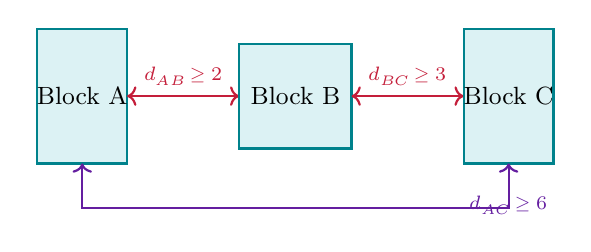
\begin{tikzpicture}[scale=0.95]
  % Block A
  \draw[draw=myteal, fill=hdrteal, thick] (0,0) rectangle (1.2,1.8) node[midway, font=\small] {Block A};
  \draw[line, <->, color=myred] (1.2,0.9) -- (2.7,0.9) node[midway, above, font=\scriptsize] {$d_{AB} \ge 2$};
  % Block B
  \draw[draw=myteal, fill=hdrteal, thick] (2.7,0.2) rectangle (4.2,1.6) node[midway, font=\small] {Block B};
  \draw[line, <->, color=myred] (4.2,0.9) -- (5.7,0.9) node[midway, above, font=\scriptsize] {$d_{BC} \ge 3$};
  % Block C
  \draw[draw=myteal, fill=hdrteal, thick] (5.7,0) rectangle (6.9,1.8) node[midway, font=\small] {Block C};
  
  % Direct constraint A to C
  \draw[line, <->, color=mypurple] (0.6,0.0) -- ++(0,-0.6) -- ++(5.7,0) -- (6.3,0.0) node[midway, below, font=\scriptsize] {$d_{AC} \ge 6$};
\end{tikzpicture}
\end{minipage}\hfill
\begin{minipage}{0.48\linewidth}
\centering
\textbf{Equivalent Constraint Graph:}\par\noindent
\vspace{8pt}
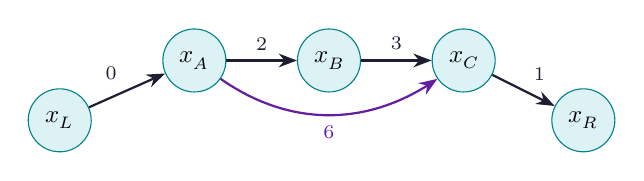
\begin{tikzpicture}[scale=0.95, gnode/.style={circle, draw=myteal, fill=hdrteal, minimum size=0.8cm, font=\small}]
  \node[gnode] (L) at (0,0) {$x_L$};
  \node[gnode] (A) at (1.8,0.8) {$x_A$};
  \node[gnode] (B) at (3.6,0.8) {$x_B$};
  \node[gnode] (C) at (5.4,0.8) {$x_C$};
  \node[gnode] (R) at (7.0,0) {$x_R$};

  \draw[arrow] (L) -- node[midway, above left, font=\scriptsize] {0} (A);
  \draw[arrow] (A) -- node[midway, above, font=\scriptsize] {2} (B);
  \draw[arrow] (B) -- node[midway, above, font=\scriptsize] {3} (C);
  \draw[arrow] (C) -- node[midway, above right, font=\scriptsize] {1} (R);
  \draw[arrow, bend right=35, color=mypurple] (A) to node[midway, below, font=\scriptsize] {6} (C);
\end{tikzpicture}
\end{minipage}
\end{tcolorbox}

% ===============================================================================
\section{Circuit Placement}
% ===============================================================================

\subsection{1. Force-Directed Placement}
Force-Directed Placement models the placement problem as a physical system of springs (Hooke's law). Standard cells are point masses, and interconnects are springs.
\begin{itemize}[leftmargin=*, itemsep=2pt]
  \item \textbf{Spring Force Formula:} The force between cell $i$ and cell $j$ connected by a net with weight $w_{ij}$ is:
        \begin{equation}
          F_{ij} = w_{ij} (x_j - x_i)
        \end{equation}
  \item \textbf{Equilibrium Equations:} The total force on cell $i$ must be zero:
        \begin{equation}
          \sum_{j} w_{ij} (x_j - x_i) = 0 \quad \Rightarrow \quad x_i \sum_{j} w_{ij} - \sum_{j} w_{ij} x_j = 0
        \end{equation}
        This is written in matrix form as $C x = f$, where $C$ is the connectivity Laplacian matrix. Solving this system gives optimal cell coordinates that minimize quadratic wirelength.
\end{itemize}

\subsection{2. Min-Cut Placement (Breuer's Algorithm)}
Min-Cut placement uses a top-down divide-and-conquer strategy:
\begin{enumerate}[leftmargin=*, itemsep=2pt]
  \item Start with the entire chip area containing all standard cells.
  \item Bisect the chip area horizontally or vertically.
  \item Use a graph partitioning algorithm (e.g. Kernighan-Lin) to partition the cells into two subsets, minimizing the number of nets crossing the cut line.
  \item Recursively apply this bisection to the sub-regions until each region contains only one or a few cells.
\end{enumerate}

% ===============================================================================
\section{Circuit Partitioning}
% ===============================================================================

\begin{tcolorbox}[defbox, title={Circuit Partitioning}]
  \textbf{Circuit Partitioning} is the process of dividing a circuit (modeled as a graph or hypergraph) into two or more sub-circuits (partitions) such that the size of each partition is balanced (respecting capacity limits) and the number of connections between the partitions (the cut size) is minimized.
\end{tcolorbox}

\subsection{Circuit Representation}
Before applying partitioning or placement algorithms, the physical netlist must be modeled mathematically. The common circuit representation models are:
\begin{itemize}[leftmargin=*, itemsep=3pt]
  \item \textbf{Standard Graph ($G = (V, E)$):} Vertices $V$ represent electronic components (gates, standard cells), and edges $E$ represent electrical connections. While simple, graphs are limited because they can only model two-terminal nets.
  \item \textbf{Hypergraph ($H = (V, E_h)$):} A generalization of a graph where a hyperedge $e \in E_h$ can connect any subset of vertices. Hypergraphs are the most accurate model for circuits because actual nets often connect three or more pins.
  \item \textbf{Connectivity Matrix ($C$):} An $n \times n$ symmetric matrix where the entry $c_{ij}$ represents the connectivity strength (number of common nets) between component $i$ and component $j$.
  \item \textbf{Laplacian Matrix ($L$):} Formulated as $L = D - C$, where $D$ is the diagonal degree matrix ($d_{ii} = \sum_j c_{ij}$). The Laplacian matrix is central to analytical, force-directed placement algorithms, converting wirelength minimization into a system of linear equations ($L x = f$).
\end{itemize}

\subsection{Kernighan-Lin (KL) Algorithm}
The KL algorithm is an iterative, heuristic bipartitioning algorithm for undirected graphs. It starts with an initial balanced partition $(A, B)$ of size $n$ each ($|V| = 2n$), and swaps pairs of nodes to reduce the cut cost.

\subsubsection{Mathematical Formulations}
For each node $a \in A$:
\begin{itemize}[leftmargin=*, itemsep=2pt]
  \item \textbf{External Cost ($E_a$):} Connection cost to nodes in the other partition: $E_a = \sum_{y \in B} c_{ay}$.
  \item \textbf{Internal Cost ($I_a$):} Connection cost to nodes in the same partition: $I_a = \sum_{x \in A} c_{ax}$.
  \item \textbf{D-Value ($D_a$):} Difference representing the priority of node $a$ for swapping:
        \begin{equation}
          D_a = E_a - I_a
        \end{equation}
  \item \textbf{Gain ($g_{ab}$):} The net reduction in cut cost if node $a \in A$ and $b \in B$ are swapped:
        \begin{equation}
          g_{ab} = D_a + D_b - 2c_{ab}
        \end{equation}
        where $c_{ab}$ is the weight of the edge between $a$ and $b$.
\end{itemize}

\begin{tcolorbox}[tikzbox, title={Kernighan-Lin Swapping Concept}]
\centering
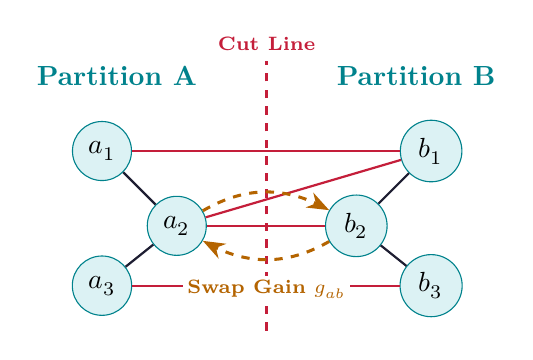
\begin{tikzpicture}[scale=0.95]
  % Partition boundary
  \draw[dashed, color=myred, line width=1pt] (3,-1.2) -- (3,2.4) node[above, font=\scriptsize\bfseries] {Cut Line};
  \node[font=\bfseries\color{myteal}] at (1,2.2) {Partition A};
  \node[font=\bfseries\color{myteal}] at (5,2.2) {Partition B};

  % Nodes in A
  \node[circle, draw=myteal, fill=hdrteal, minimum size=0.6cm] (a1) at (0.8,1.2) {$a_1$};
  \node[circle, draw=myteal, fill=hdrteal, minimum size=0.6cm] (a2) at (1.8,0.2) {$a_2$};
  \node[circle, draw=myteal, fill=hdrteal, minimum size=0.6cm] (a3) at (0.8,-0.6) {$a_3$};
  
  % Nodes in B
  \node[circle, draw=myteal, fill=hdrteal, minimum size=0.6cm] (b1) at (5.2,1.2) {$b_1$};
  \node[circle, draw=myteal, fill=hdrteal, minimum size=0.6cm] (b2) at (4.2,0.2) {$b_2$};
  \node[circle, draw=myteal, fill=hdrteal, minimum size=0.6cm] (b3) at (5.2,-0.6) {$b_3$};

  % Connections within A
  \draw[line] (a1) -- (a2);
  \draw[line] (a2) -- (a3);

  % Connections within B
  \draw[line] (b1) -- (b2);
  \draw[line] (b2) -- (b3);

  % Cut Connections
  \draw[line, color=myred] (a1) -- (b1);
  \draw[line, color=myred] (a2) -- (b2);
  \draw[line, color=myred] (a2) -- (b1);
  \draw[line, color=myred] (a3) -- (b3);

  % Swap indication
  \draw[arrow, bend left, color=myamber, dashed, line width=1.1pt] (a2) to (b2);
  \draw[arrow, bend left, color=myamber, dashed, line width=1.1pt] (b2) to (a2);
  \node[color=myamber, font=\scriptsize\bfseries, fill=white, inner sep=1.5pt] at (3, -0.65) {Swap Gain $g_{ab}$};
\end{tikzpicture}
\tcblower
Swap gain formula: $g_{ab} = D_a + D_b - 2c_{ab}$. If swapped, the cut size decreases by $g_{ab}$.
\end{tcolorbox}

\subsubsection{Algorithmic Steps for One Pass}
\begin{enumerate}[leftmargin=*, itemsep=2pt]
  \item Mark all vertices as \textit{unlocked}.
  \item Compute $D$-values for all vertices in $A$ and $B$.
  \item For $i = 1$ to $n$:
    \begin{itemize}[leftmargin=*, label=$\bullet$, itemsep=1.5pt]
      \item Choose an unlocked pair $(a_i, b_i) \in A \times B$ that maximizes $g_i = D_{a_i} + D_{b_i} - 2c_{a_i b_i}$.
      \item Lock $a_i$ and $b_i$ (they cannot be swapped again in this pass).
      \item Update $D$-values of remaining unlocked neighbors:
            \begin{align*}
              D'_x &= D_x + 2c_{x a_i} - 2c_{x b_i} \quad \text{for } x \in A \\
              D'_y &= D_y + 2c_{y b_i} - 2c_{y a_i} \quad \text{for } y \in B
            \end{align*}
    \end{itemize}
  \item Find the step $k$ that maximizes the cumulative gain $G_k = \sum_{i=1}^{k} g_i$.
  \item If $G_k > 0$, swap the sets $\{a_1, \ldots, a_k\}$ and $\{b_1, \ldots, b_k\}$ permanently and start a new pass. If $G_k \le 0$, terminate (no further improvement possible).
\end{enumerate}

\begin{tcolorbox}[examplebox, title={Kernighan-Lin Step-by-Step Example}]
\Q{Problem:} Consider a graph with $V = \{1, 2, 3, 4, 5, 6\}$ and edges $E = \{(1,2), (1,3), (1,4), (2,5), (3,6), (4,5), (5,6)\}$. The initial partitions are $A = \{1, 2, 3\}$ and $B = \{4, 5, 6\}$. Find the gains and update the partitions.

\textbf{Solution:}\par\noindent
\textbf{Step 1: Compute initial D-values:}
\begin{itemize}[leftmargin=*, itemsep=1pt]
  \item Node 1: $E_1 = c_{14} = 1$; $I_1 = c_{12} + c_{13} = 2$. $\Rightarrow D_1 = 1 - 2 = -1$.
  \item Node 2: $E_2 = c_{25} = 1$; $I_2 = c_{21} = 1$. $\Rightarrow D_2 = 1 - 1 = 0$.
  \item Node 3: $E_3 = c_{36} = 1$; $I_3 = c_{31} = 1$. $\Rightarrow D_3 = 1 - 1 = 0$.
  \item Node 4: $E_4 = c_{41} = 1$; $I_4 = c_{45} = 1$. $\Rightarrow D_4 = 1 - 1 = 0$.
  \item Node 5: $E_5 = c_{52} = 1$; $I_5 = c_{54} + c_{56} = 2$. $\Rightarrow D_5 = 1 - 2 = -1$.
  \item Node 6: $E_6 = c_{63} = 1$; $I_6 = c_{65} = 1$. $\Rightarrow D_6 = 1 - 1 = 0$.
\end{itemize}

\textbf{Step 2: Calculate gains $g_{ij} = D_i + D_j - 2c_{ij}$ for unlocked pairs:}
\begin{itemize}[leftmargin=*, itemsep=1pt]
  \item $g_{14} = D_1 + D_4 - 2c_{14} = -1 + 0 - 2(1) = -3$
  \item $g_{15} = D_1 + D_5 - 2c_{15} = -1 - 1 - 0 = -2$
  \item $g_{24} = D_2 + D_4 - 2c_{24} = 0 + 0 - 0 = 0$
  \item $g_{25} = D_2 + D_5 - 2c_{25} = 0 - 1 - 2(1) = -3$
  \item $g_{36} = D_3 + D_6 - 2c_{36} = 0 + 0 - 2(1) = -2$
  \dots
\end{itemize}
The maximum gain is $g_1 = g_{24} = 0$ (swap Node 2 and Node 4).
Lock Node 2 and Node 4.

\textbf{Step 3: Update D-values for remaining unlocked nodes $\{1, 3\}$ and $\{5, 6\}$:}
\begin{itemize}[leftmargin=*, itemsep=1pt]
  \item $D'_1 = D_1 + 2c_{12} - 2c_{14} = -1 + 2(1) - 2(1) = -1$
  \item $D'_3 = D_3 + 2c_{32} - 2c_{34} = 0 + 0 - 0 = 0$
  \item $D'_5 = D_5 + 2c_{54} - 2c_{52} = -1 + 2(1) - 2(1) = -1$
  \item $D'_6 = D_6 + 2c_{64} - 2c_{62} = 0 + 0 - 0 = 0$
\end{itemize}

Calculate gains for the second step:
\begin{itemize}[leftmargin=*, itemsep=1pt]
  \item $g_{15} = D'_1 + D'_5 - 2c_{15} = -1 - 1 - 0 = -2$
  \item $g_{16} = D'_1 + D'_6 - 2c_{16} = -1 + 0 - 0 = -1$
  \item $g_{35} = D'_3 + D'_5 - 2c_{35} = 0 - 1 - 0 = -1$
  \item $g_{36} = D'_3 + D'_6 - 2c_{36} = 0 + 0 - 2(1) = -2$
\end{itemize}
Choose swap pair (1, 6) or (3, 5) with $g_2 = -1$.
Let's select (3, 5) to swap. Lock $\{3, 5\}$.
After calculating the remaining gain, we determine that cumulative gain $G_k$ is not positive. The optimal choice is to not make any swaps, or restart with a different initial partition.
\end{tcolorbox}

\subsection{Fiduccia-Mattheyses (FM) Partitioning Algorithm}
The FM algorithm is an extension of the KL algorithm that partitions hypergraphs.
Key enhancements over KL:
\begin{itemize}[leftmargin=*, itemsep=2pt]
  \item \textbf{Single Node Moves:} Instead of swapping pairs, it moves one cell at a time from its partition to another. This allows handling partitions of unequal sizes.
  \item \textbf{Linear Time Complexity:} Time complexity is reduced to $O(|E|)$ per pass by using a bucket array data structure to select the unlocked cell with the maximum gain in $O(1)$ time.
\end{itemize}

\newpage

% ═══════════════════════════════════════════════════════════════════════════════
% QUICK REVISION PAGE
% ═══════════════════════════════════════════════════════════════════════════════
\begin{center}
  {\large\bfseries\color{myred} Quick Revision — Module 2}\\[3pt]
  {\small\color{mydark} Partitioning, Placement \& Compaction $|$ PE-EC802C}
\end{center}
\noindent{\color{myred}\rule{\linewidth}{1.2pt}}
\vspace{8pt}

\begin{tcolorbox}[formulabox, title={\textbf{Key Formulas and Metrics at a Glance}}]
\renewcommand{\arraystretch}{1.35}
\begin{tabularx}{\linewidth}{B{5.0cm} X}
  Constraint Spacing & $x_j - x_i \ge d_{ij} \quad (\text{directed edge } v_i \rightarrow v_j \text{ with weight } d_{ij})$ \\[4pt]
  Force-Directed Coordinate & $x_i = \dfrac{\sum_{j} w_{ij} x_j}{\sum_{j} w_{ij}} \quad (\text{equilibrium position})$ \\[4pt]
  Kernighan-Lin Gain & $g_{ab} = D_a + D_b - 2c_{ab} \quad (D_k = E_k - I_k \text{ node priority})$
\end{tabularx}
\end{tcolorbox}

\vspace{6pt}

\begin{tcolorbox}[defbox, title={\textbf{One-Line Definitions}}]
\begin{itemize}[leftmargin=*, itemsep=3pt, topsep=0pt]
  \item \textbf{1D Compaction:} Compressing elements along one axis in a single step (either horizontal or vertical).
  \item \textbf{Constraint Graph:} A directed graph representing layout elements as vertices and spacing rules as weighted edges.
  \item \textbf{Hypergraph:} A graph where a hyperedge can connect any number of vertices, used to model multi-terminal nets.
  \item \textbf{Laplacian Matrix:} A matrix representation of connectivity used in force-directed placements.
  \item \textbf{Cut Size:} The number of nets or edges crossing the boundaries separating different partitions.
  \item \textbf{Gain (KL):} The net reduction in the cut cost resulting from swapping two nodes between partitions.
  \item \textbf{FM Algorithm:} A linear-time hypergraph partitioning algorithm that moves a single node at a time.
\end{itemize}
\end{tcolorbox}

\vspace{6pt}

\begin{tcolorbox}[exambox, title={\textbf{Frequently Asked / Viva Questions}}]
\begin{enumerate}[leftmargin=*, topsep=0pt, label=\textbf{Q\arabic*.}, itemsep=6pt]
  \item \Q{What are spacing and width rules in layout compaction?}
        Width rules dictate the minimum dimension of a layout wire or layer (to prevent breaks due to line width tolerances). Spacing rules define the minimum distance between two separate features (to prevent short circuits due to lithographic misalignment).
        
  \item \Q{How is a layout feature mapped to a constraint graph during compaction?}
        Each vertical layout edge (for X-compaction) or horizontal layout edge (for Y-compaction) is represented as a vertex. The minimum design rule spacing between the two edges is represented as a directed, weighted edge connecting the vertices.
        
  \item \Q{What is the difference between a graph and a hypergraph?}
        In a standard graph, each edge connects exactly two vertices. In a hypergraph, an edge (hyperedge) can connect a subset containing any number of vertices. Circuits are modeled as hypergraphs because a single signal line (net) typically connects multiple component pins.
        
  \item \Q{Why does the KL partitioning algorithm lock swapped nodes?}
        If swapped nodes were not locked, the algorithm could end up in an infinite loop by swapping the same nodes back and forth. Locking them guarantees that every node is swapped at most once per pass, ensuring termination in exactly $n$ steps.
        
  \item \Q{What is the purpose of the virtual source and sink nodes in constraint graphs?}
        The virtual source node ($x_{\text{left}}$) represents the left edge of the chip boundary ($x = 0$). The virtual sink node ($x_{\text{right}}$) represents the right boundary. The longest path from source to sink determines the minimum width of the entire compacted layout.
        
  \item \Q{How does force-directed placement handle cell overlaps?}
        Force-directed placement minimizes total quadratic wirelength, which pulls all connected cells toward the center of the chip, causing significant cell overlaps. To resolve overlaps, placement tools follow the force calculation step with slot assignment or recursive partitioning.
        
  \item \Q{Explain the role of the bucket array structure in the FM algorithm.}
        The FM algorithm uses a bucket array to index unlocked cells by their gain values. Cells with the same gain are linked together. This data structure allows the cell with the maximum gain to be found and retrieved in $O(1)$ constant time, enabling overall linear time complexity.
        
  \item \Q{What are the limitations of the KL algorithm?}
        (1) It only works on standard graphs, not hypergraphs. (2) It can only handle partitions of equal sizes. (3) Its time complexity is $O(n^3)$ per pass, which is too slow for modern circuits containing millions of nodes.
        
  \item \Q{Why is quadratic wirelength used in force-directed placement instead of linear wirelength?}
        Quadratic wirelength uses a squared distance metric ($d^2$), which can be formulated as a set of linear equations. Solving linear equations is mathematically straightforward and fast (using matrix solvers). Linear wirelength optimization requires absolute values ($|d|$), which cannot be solved directly in a single step.
        
  \item \Q{What is a connectivity matrix, and how does it represent net weights?}
        A connectivity matrix $C$ is a matrix where the entry $C_{ij}$ represents the number of nets connecting cell $i$ and cell $j$. Higher values of $C_{ij}$ indicate a stronger connection, which generates a stronger attractive force during force-directed placement, pulling the cells closer together.
\end{enumerate}
\end{tcolorbox}

\vspace{6pt}

\begin{tcolorbox}[tikzbox, title={\textbf{Comparison Snapshot}}]
\textbf{1D vs. 2D Compaction:}\par\vspace{6pt}\noindent
{\renewcommand{\arraystretch}{1.35}%
\begin{tabularx}{\linewidth}{|B{3.2cm}|Y|Y|}
\hline
\textbf{Feature} & \textbf{1D Compaction} & \textbf{2D Compaction} \\
\hline
Squeezing Axis & Squeezes sequentially (X first, then Y). & Squeezes simultaneously in both X and Y. \\
\hline
Complexity & Polynomial time ($O(n \log n)$), very fast. & NP-complete, computationally intractable. \\
\hline
Optimality & Suboptimal (leaves redundant space). & Achieves absolute minimum silicon area. \\
\hline
\end{tabularx}}

\vspace{12pt}
\textbf{KL vs. FM Partitioning:}\par\vspace{6pt}\noindent
{\renewcommand{\arraystretch}{1.35}%
\begin{tabularx}{\linewidth}{|B{3.2cm}|Y|Y|}
\hline
\textbf{Feature} & \textbf{Kernighan-Lin (KL) Algorithm} & \textbf{Fiduccia-Mattheyses (FM) Algorithm} \\
\hline
Circuit Model & Standard graph (edges connect two nodes). & Hypergraph (hyperedges connect multiple nodes). \\
\hline
Move Strategy & Swaps pairs of nodes ($a \in A, b \in B$). & Moves a single node at a time. \\
\hline
Time Complexity & $O(n^3)$ per pass. & $O(|E|)$ (linear time) per pass. \\
\hline
Partition Size & Forces strictly equal sizes. & Supports flexible/unbalanced partition sizes. \\
\hline
\end{tabularx}}
\end{tcolorbox}

\end{document}
